\section{Il programma: descrizione e scelta dei parametri}
Per semplicit\`a e alleggerire i calcoli ho impostato $\hbar=1$, 
Gli eseguibili compilabili dal Makefile sono i seguenti, nei commenti \`e spiegato come eseguirli:
\lstinputlisting[language=make, firstline = 17, lastline = 40,frame = single]{../Makefile}
\begin{itemize}
\item Il programma pi\`u semplice (\textit{single}) \`e composto da un blocco \textit{impostazioni} che carica i file con le informazioni sulla simulazione, crea la trimatrice e le condizioni iniziali ,e un blocco \textit{CrankSolver} che si occupa di svolgere risolvere il sistema passo per passo (nel nostro caso non avendo potenziali che dipendono dal tempo la riduzione della trimatrice viene fatta solo una volta, nella costruzione del \textit{CrankSolver}).
  Ho scelto di impostare il \textit{CrankSolver} in modo che contenga solo i punti del passo attuale perch\'e l'elevato numero di punti rischia di intasare la memoria del sistema piuttosto in fretta: i punti calcolati vengono salvati su un file in una cartella ``./results'', che deve essere creata prima di lanciare l'eseguibile, il numero di punti e la frequenza di essi viene deciso nei file di impostazione.
\item \textit{experiment} funziona come \textit{single} ma ripete la simulazione per ogni potenziale che trova nella lista \textit{namelist.txt} nella cartella in cui viene chiamato.
\item \textit{drawer}, \textit{analisi}, \textit{CVD} e \textit{preview} sono i programmi che vengono utilizzati nell'analisi delle simulazioni:
  \begin{itemize}
  \item \textit{analisi} carica i file  \textit{.dat} contenuti in \textit{namelist.txt} e ne fa varie analisi (plot degli errori, plot degli integrali nella prima/seconda met\`a del dominio, plot della posizione dei massimi).
  \item \textit{drawer} fa le stesse operazioni di analisi, ma relative a un singolo file \textit{.dat}, inoltre mostra l'evoluzione dell'onda grazie a un \textit{TGraph2D}.
  \item \textit{CVD} mostra i vari potenziali il cui elenco \`e contenuto nel file \textit{infonamelist.txt}, carica le impostazioni del dominio da un file \textit{settings.set} dato.
  \item \textit{preview} deve essere lanciato con \textit{./runscript.sh} (che imposta \lstinline[language = bash]|export LD_LIBRARY_PATH=$LD_LIBRARY_PATH:./|) \`e una piccola interfaccia grafica che permette di fare qualche analisi sui risultati della simulazione.
  \end{itemize}
\end{itemize}
\begin{figure}[htb]
  \centering
  \begin{tikzpicture}[mindmap, concept color = orange!50,every node/.style = {concept}]
    \node (main){main}
    child[concept color = orange,grow = 180]{node(impostazioni){Impostazioni}
      child[concept color = red, grow = 200]{node {file\\potenziale}}
      child[concept color = red, grow = 20]{node (pot){Potenziale}
	child[concept color = yellow, grow = right, level 2 concept]{node(tridiag){matrice\\tridiagonale}}}
      child[concept color = blue!75, grow = 140]{node {file\\onda}}
      child[concept color = blue!75, grow = -20]{node (CC){CC}}
      child[concept color = blue!75, grow = -60]{node (CI){CI}}
      child[concept color = green, grow = 240]{node(set) {file\\settings}}
      child[concept color = green, grow = 60]{node (con){passi e \\costanti}
	child[concept color = green, grow = right] {node(eta){$\eta$}}}
    }
    child[concept color = orange,grow =0] {node (Solver) {CrankSolver}}
    child[concept color = red!50,grow = down]{node(out){output}};
    \path(tridiag) to[circle connection bar switch color = from (yellow) to (green)](eta);
    \path(tridiag) to[circle connection bar switch color = from (yellow) to (orange)](Solver);
    \path(tridiag) to[circle connection bar switch color = from (yellow) to (blue!75)](CC);
    \path(Solver) to[circle connection bar switch color = from (orange) to (blue!75)](CI);
    \path(Solver) to[circle connection bar switch color = from (orange) to (red!50)](out);
    \path(set) to[circle connection bar switch color = from (green) to (red!50)](out);
  \end{tikzpicture}
  \caption{Collegamenti tra i blocchi del programma}
\end{figure}

\subsection{Impostazioni}
Il programma pi\`u semplice, compilabile con \lstinline|$> make single| carica i dati da tre file di impostazioni, in cui viene alternata una riga di commento, anticipata da un ``\textit{\#}'' e una con i valori dell'impostazione, l'ordine \`e importante e il commento non deve contenere spazi.

Il file generale delle impostazioni:
\lstinputlisting[frame = single,caption=Impostazioni principali]{../settings.set}\label{lst:settings}
In questo file fornisco i parametri principali della simulazione, quelli che ho previsto che avrei cambiato pi\`u di rado durante la simulazione. ``\textit{\#massa} e ``\textit{\#lunghezza}'' sono ovvi, ``\textit{\#tmax}'' \`e il tempo a cui si ferma la simulazione. L'opzione ``\textit{\#Ndipende\_da\_intervallo=0}'' se impostata uguale a $0$ fa s\`i che il numero di passi (spaziali e temporali) venga calcolato conoscendo la lunghezza totale e il passo, se impostata diversa da $0$ invece fa s\`i che il programma calcoli il passo a partire dalla lunghezza totale e il numero di punti voluti. Le opzioni ``\textit{\#timeskip}'' e ``\textit{\#spaceskip}'' servono nel momento di salvare i risultati: il primo imposta ogni quanti passi temporali esportare il vettore di punti, che vengono salvati ad intervalli decisi dal secondo parametro. Il parametro ``\textit{\#precisione}'' invece blocca la simulazione prima del tempo massimo se l'errore (vedi \autoref{sec:errore}) supera il valore impostato, se lo si imposta a 0 salta il controllo.

Il file delle condizioni iniziali:
\lstinputlisting[frame = single,caption=Impostazioni CI]{../gauss.set}
Il primo parametro deve essere una lettera e serve a indicare al programma la forma del pacchetto d'onda nelle condizioni iniziali, se viene scritto ``\textit{b}'' il programma disegner\`a la funzione ``bump'' con parametri presi dalla riga successiva, nell'ordine ``altezza del massimo'', ``larghezza'' e ``punto del massimo''; negli altri casi una gaussiana con i parametri ``altezza'', ``deviazione standard'' e ``punto medio''. I due set successivi alle impostazioni dell'onda riguardano le condizioni al contorno, la prima che pu\`o essere $0$, $1$ o $2$ indica il tipo di condizione, rispettivamente Dirichlet, Neumann o Robin sulla stessa riga il primo numero indica il valore della funzione, della derivata o della combinazione lineare, il terzo parametro viene solo utilizzata da Robin ed \`e il peso della funzione\footnote{Per Dirichlet $f(\bar x) = var$, per Neumann $\lr.|{\de{f}x}_{\bar x} = var$ e per Robin $\lr.|{\de{f}x}_{\bar x} + (pesorobin) f(\bar x) = var$}
L'ultima impostazione \`e l'energia con cui si vuole lanciare l'onda.

Il file del potenziale:
\lstinputlisting[frame = single,caption=Impostazioni potenziale]{../potenziale.set}
Il primo parametro imposta la forma del potenziale, che pu\`o essere una gaussiana, un ``bump'', un rettagolo oppure un salto.
Nella riga successiva il primo parametro imposta l'altezza  del punto pi\`u alto del potenziale, se messo a 0 dice all'algoritmo di calcolare l'evoluzione in assenza di potenziale, il secondo parametro indica il centro della funzione se \`e pari, oppure la posizione del salto, l'ultimo parametro indica la larghezza o la deviazione standard del potenziale non viene utilizzato se la forma \`e il salto.

\subsection{Condizioni iniziali}
La mia idea \`e di simulare l'evoluzione di un pacchetto di onde piane quindi nella forma
\begin{equation}
  \Psi(x,t) = \psi(x,t)e^{ik_0x-\omega t} \to \Psi(x,0) = \psi(x,0)e^{ik_0x}
\end{equation}
O, meglio:
\begin{equation}
  \Psi(x,t) = \frac{1}{\sqrt{2\pi}}\int_{-\infty}^{+\infty} F(k) e^{ikx-\omega t}\df k
\end{equation}
Dato che utilizzer\`o un pacchetto  di forma gaussiana, nel programma non far\`o mai l'integrale in quanto la trasformata di Fourier di una gaussiana \`e una gaussiana.
Avr\`o:
\begin{equation}
  \Psi(x,0) = Ae^{-\frac{\lrt{x-x_0}^2}{2\sigma}}e^{ikx}
\end{equation}

%\begin{equation}
%\Psi(x,t) = Ae^{-\frac{\lrt{x-x_0-ct}^2}{2\sigma}}e^{ikx-ickt}
%\end{equation}

\begin{figure}[hbt]
  \centering
  \begin{tikzpicture}
    \draw[->] (-2,0) -- (2,0) node[right] {};
    \draw[->] (0,-1.2) -- (0,1.3) node[above] {};
    \node[below] at (1,0){1};
    \node[left] at (0,1){1};
    \node[right, color=red] at(1.5,0.8){Im};
    \node[right, color=blue] at(1.5,1.1){Re};
    \node[right] at(1.5,1.4){abs};
    \draw[domain=-2:2, samples =501]   plot[id=ini] function{exp(-x*x)};
    \draw[domain=-2:2, samples =501,blue]  plot[id=iniR] function{exp(-x*x)*cos(7*x)};
    \draw[domain=-2:2, samples =501,red] plot[id=iniI] function{exp(-x*x)*sin(7 *x)};
  \end{tikzpicture}
  \caption{Le condizioni iniziali, con $x_0=0,\ A=1,\ \sigma = 1$ e $k=7$}
\end{figure}
Dove $x_0$ \`e il punto del massimo dell'onda, $\sigma$ la sua deviazione standard e $A$ un parametro che cambia l'altezza del massimo.
La velocit\`a di gruppo $k$ dipende dall'energia secondo la relazione di dispersione $k(E) = \sqrt{\frac{2m}{\hbar^2}E}$, tenendo conto che nelle condizioni iniziali le particelle del treno sono da considerarsi libere (ovvero non sono influenzate dal potenziale nel punto in cui le ho depositate).

Poich\'e la forma dell'onda \`e moltiplicata per $e^{ikx}$ e deve essere discretizzata devo come minimo scegliere un passo che non cada in problemi di aliasing, e quindi campionare con una frequenza superiore a $k$, ovvero il passo deve essere pi\`u piccolo di $1/k$.

La discretizzazione delle condizioni iniziali, gaussiane:
\begin{equation}
  CI\lrq{j}= Ae^{-\frac{\lrt{j*\df x-x_0}^2}{2\sigma}+i k j*\df x}
\end{equation}

\subsection{Lancio senza potenziale: errore}\label{sec:errore}
Prima di tutto voglio effettuare qualche simulazione senza potenziale per poter osservare come si comporta l'onda.

Ho bisogno di definire un ``errore'' per capire quanto la simulazione possa essere andata a buon fine:
la mia scelta \`e stata di utilizzare la norma della funzione, ricordando che le funzioni d'onda sono $L^2$ e quindi la loro norma \`e  $\lr||f^2=\int_X\lr||f^2d\mu$.
Ho utilizzato la definizione dell'integrale discreto di Simpson, il che mi limita a poter fare solo simulazioni con un numero di passi pari (e in particolare multipli di 4 per aver un integrale preciso anche quando calcolo l'integrale solo nella prima o seconda met\`a del dominio) nello spazio.

Nella simulazione blocco il calcolo se la norma della funzione si discosta troppo dalla norma delle condizioni iniziali, il limite viene scelto nel file delle impostazioni.

\begin{figure}[hbt]
	\centering
	\begin{subfigure}[b]{0.3\textwidth}
		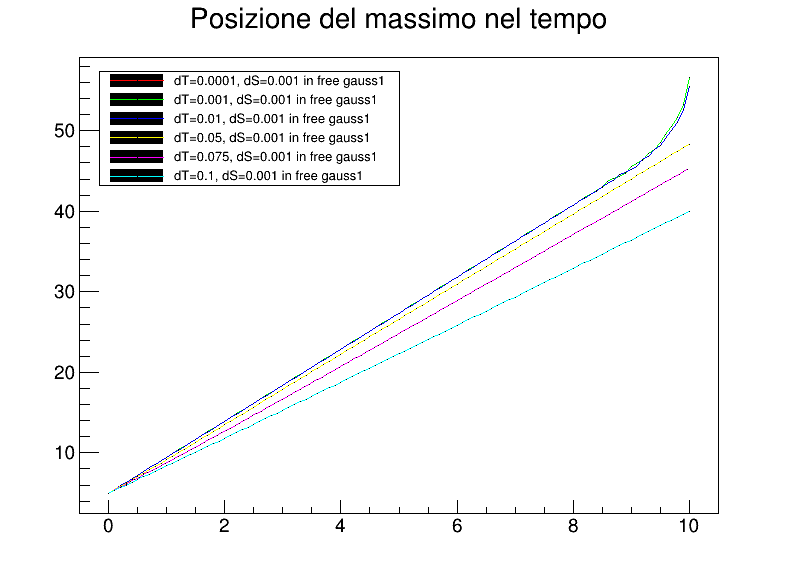
\includegraphics[width=\textwidth]{IMG/v_g1_0001}
		\caption[Differenze in 0.001]{Le differenze per $dS = 0.001$}
	\end{subfigure}
	~
	\begin{subfigure}[b]{0.3\textwidth}
		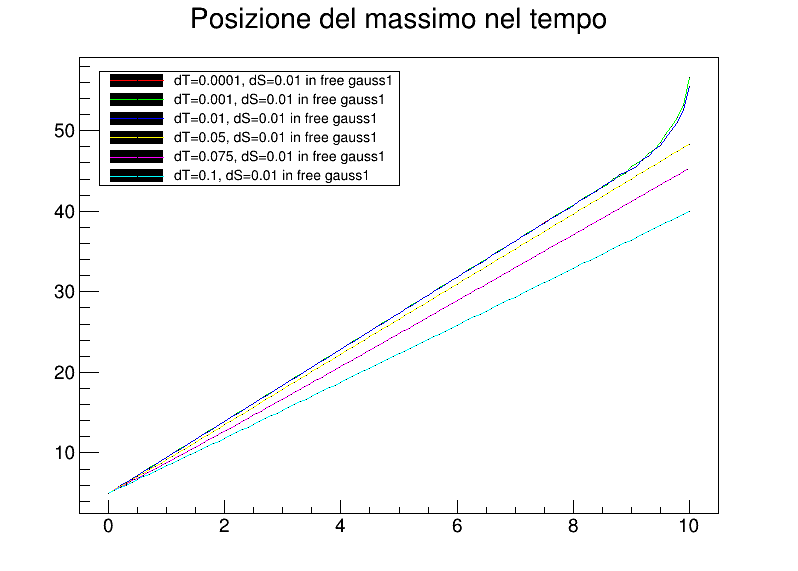
\includegraphics[width=\textwidth]{IMG/v_g1_001}
		\caption[Differenze in 0.01]{Le differenze per $dS = 0.01$}
	\end{subfigure}
	~
	\begin{subfigure}[b]{0.3\textwidth}
		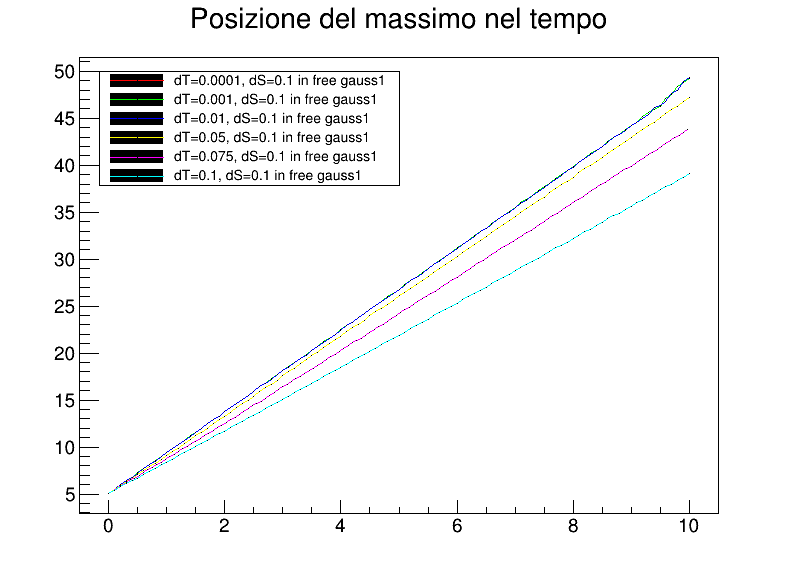
\includegraphics[width=\textwidth]{IMG/v_g1_01}
		\caption[Differenze in 0.1]{Le differenze per $dS = 0.1$}
	\end{subfigure}
	\caption{Le posizioni dei massimi nel tempo della simulazione a vari passi temporali  e spaziali}\label{fig:velocita}
\end{figure}

Per capire come impostare i parametri delle simulazioni ho effettuato diversi lanci con varie combinazioni di passo temporale e passo spaziale. Riporto i vari grafici degli errori.
Da questi lanci capisco che devo scartare l'idea di usare un passo temporale grande in quanto ho notato che le funzioni d'onda vengono ``rallentate'', come si pu\`o vedere in \autoref{fig:velocita}. Dalle figure noto che le simulazioni devono avere un passo temporale non pi\`u grande di $0.01$. Il punto in cui gli andamenti perdono l'andamento lineare e` dovuto al fatto che il pacchetto sta impattando contro il bordo del dominio e quindi inizia a rimbalzare e si iniziano a vedere le figure di interferenza.
%rifare tutto per verificare teoria!!!!!!!!!!!!!!!!!!!!!!!!!!!!!!!!!!!!!!!!!!!!!!!!!!!!!!!!!!!!!!!!!!!!!!!!!
%http://www.colorado.edu/physics/phys2170/phys2170_sp07/downloads/Gaussian.pdf
Mi aspetto che la simulazione ritorni:
\begin{equation}
%\Psi(x,t) = A(t)e^{-\frac{\lrt{x-x_0-\o t}^2}{2\sigma^2}}e^{ik\lrt{x-\o t}}
\Psi(x,t) = A(t)e^{-\frac{\lrt{x-x_0- v t}^2}{2\sigma(t)^2}}e^{ikx-\o t}
\end{equation}
dove $\o = \frac E\hbar$  e $v = \frac{p}{m} =\frac{\sqrt{2m E}}{m} $, ricordando che stiamo lavorando con pacchetti di onde piane monocromatici.
Quindi che i massimi delle onde da me simulate si spostino nel tempo seguendo la legge:
\begin{equation}
x_0(t) = x_0(0)+\sqrt{2\frac{E}{m}} t
\end{equation}
%%%%%%%%%%%%%%%%%%
%%non rispetta questo ma va confrontato con il fatto che invece rispetta la dispersione
Poi ho guardato l'errore di alcune simulazioni, scartando a priori i passi pi\`u grandi di $0.01$, \autoref{fig:fullErr} e \ref{fig:fullErrzoom}.

\begin{figure}[hbt]
  \centering
  \begin{subfigure}[b]{0.45\textwidth}
    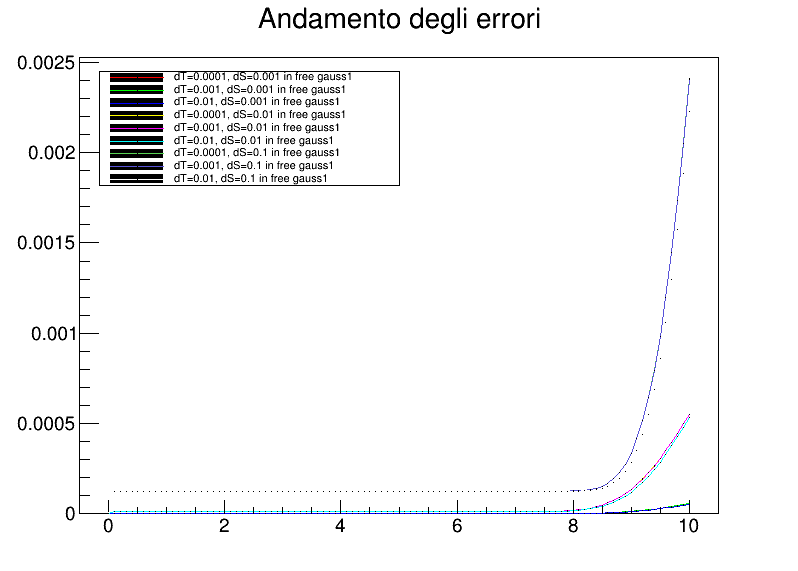
\includegraphics[width=\linewidth]{IMG/e_g1full}
    \caption[Errori completo]{Il grafico completo degli errori}\label{fig:fullErr}
  \end{subfigure}
  ~
  \begin{subfigure}[b]{0.45\textwidth}
    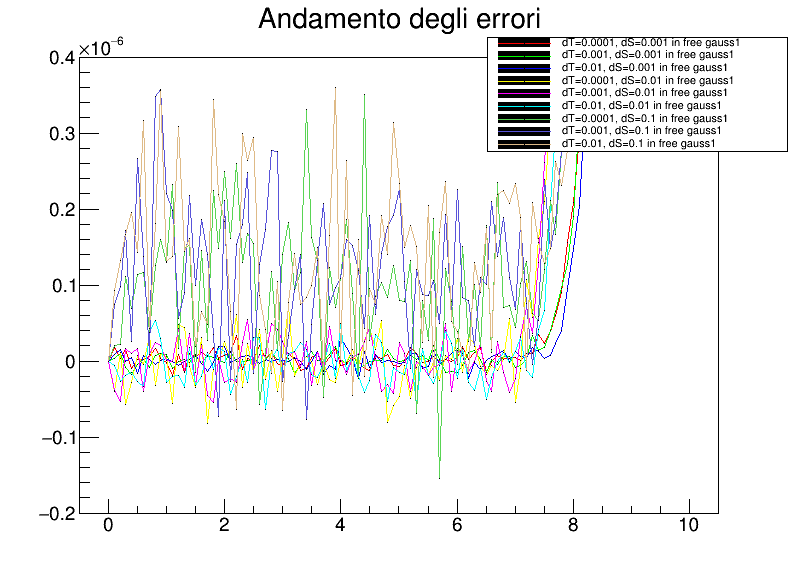
\includegraphics[width=\linewidth]{IMG/e_g1res}
    \caption[Errori zoom]{Zoom per mostrare dove la riflessione non ha influenza}\label{fig:fullErrzoom}
  \end{subfigure}
  \caption[Errori completo]{Il grafico degli errori, si vede anche quanto la riflessione influisca sul modulo della funzione.}\label{fig:Err}
\end{figure}

A questo punto ho fatto una simulazione diminuendo il tempo massimo a $6$ in modo da non avere a che fare con l'esplosione dell'errore dovuta al limite del dominio. e cosi` da poter osservare quale fosse il miglior passo spaziale. Ho fatto i lanci con due diverse condizioni iniziali (gaussiana con $\sigma$ $1$ e $2$). 

\begin{figure}[htb]
  \centering
  \begin{subfigure}[b]{0.45\textwidth}
    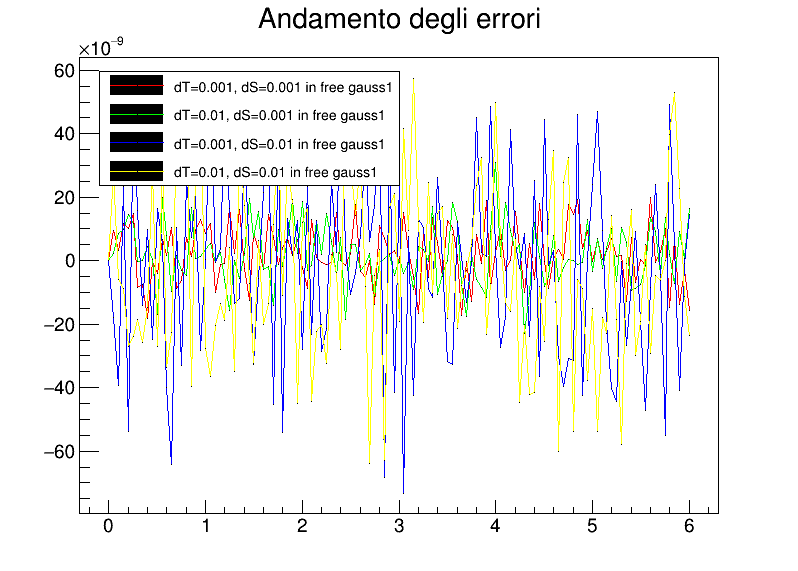
\includegraphics[width=\textwidth]{IMG/eChoosy1}
    \caption{CI: gaussiana($\sigma=2$)}
  \end{subfigure}
  ~
  \begin{subfigure}[b]{0.45\textwidth}
    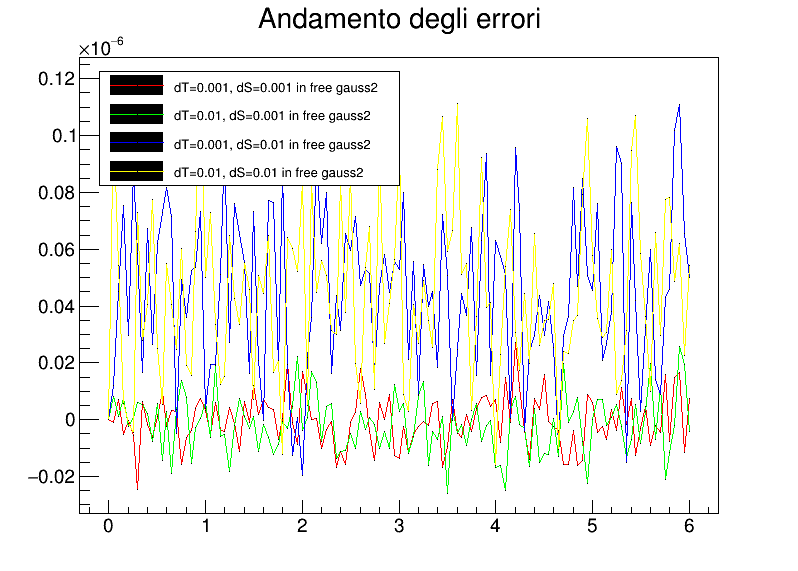
\includegraphics[width=\textwidth]{IMG/eChoosy2}
    \caption{CI: gaussiana($\sigma=2$)}
  \end{subfigure}
  \caption{I passi che mi sembravano pi\`u opportuni a confronto}\label{fig:SceltaErrori}
\end{figure}

Osservando \autoref{fig:SceltaErrori} utilizzare come passi spaziali e temporali valori compresi tra $0.01$ e $0.001$ ha un buon rapporto ``errore sulla simulazione/peso sul calcolatore'', in particolare si nota che il passo spaziale influenza di pi\`u l'errore. Ho scelto di continuare con $dT = 0.01$ e $dS = 0.005$ in quanto hanno errore molto simile a $dS = 0.001$ (\autoref{fig:sceltaPassi}) ma sono pi\`u rapidi nei calcoli (sulla mia macchina).

\begin{figure}[hbt]
  \centering
  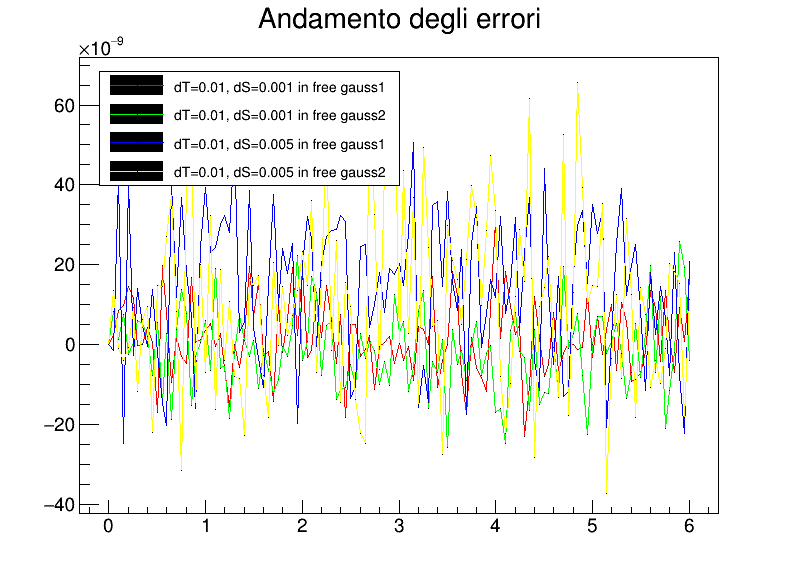
\includegraphics[width=0.7\textwidth]{IMG/sceltaPassi}
  \caption[Scelta Passi]{Gli errori dei passi che ritengo pi\`u convenienti}\label{fig:sceltaPassi}
\end{figure}

\subsection{Dispersione dei pacchetti d'onda}
%pacchetti di Airy non disperdono-> provare
\begin{figure}[htb]
  \centering
  \foreach \x in {1,3,7,10}{
    \begin{subfigure}[b]{0.4\textwidth}
      \centering
      \includegraphics[width=\textwidth]{IMG/dispersione_\x}
    \end{subfigure}
    \ifthenelse{\equal{\x}{3}}{\\}{~} 
  }
  \caption{La dispersione delle gaussiana a $\sigma =1$, in verde le condizioni iniziali}\label{fig:dispersione}
\end{figure}

La prima cosa che si pu\`o osservare nelle simulazioni (e in particolare in \autoref{fig:dispersione}) \`e la dispersione dell'onda, ovvero il pacchetto si allarga nel tempo. Questa \`e una caratteristica dell'equazione di Schr\"{o}dinger, in quanto la sua forma \`e appunto quella di una qualsiasi equazione che descriva la dispersione.

Voglio calcolare la teoria di questo fenomeno per poterlo confrontare con i risultati che ho ottenuto nelle prime simulazioni.
Per ottenere la soluzione dell'equazione con condizioni iniziali $\psi\lrt{x,0}=e^{-\frac{x^2}{2\sigma^2}}$ si passa dalla trasformata di Fourier spaziale $\hat\psi\lrt{x,0}=\sqrt{2\pi\sigma^2} e^{-\frac{k^2 \sigma^2}2}$, che porta ad avere la funzione, con dipendenza temporale:

\begin{equation}
  \hat{\psi}\lrt{k,t} = \sqrt{2\pi\sigma^2} e^{-\frac{k^2 \sigma^2}2} e^{-i\frac E\hbar t} =
  \sqrt{2\pi\sigma^2} e^{-\frac{k^2 \sigma^2}2} e^{-i\frac {\hbar^2 k^2/2m}\hbar t} = 
  \sqrt{2\pi\sigma^2} e^{-k^2\frac{\lrt{\sigma^2+i\hbar t/m}}2 }
\end{equation}
e poi ritrasformando:
\begin{equation}
  \psi\lrt{x,t} = \frac{\sigma}{\sqrt{\sigma^2 + i\hbar t /m}}
  e^{-\frac{k^2}{2\lrt{\sigma + i\hbar t/m}}}
\end{equation}
ora calcolo il valore assoluto della funzione:
\begin{equation}
  \lr||{\psi\lrt{x,t}} = \frac{\sigma}{\sqrt[4]{\sigma^4 + \lrt{\hbar t /m}^2}}
  e^{-\frac{k^2}2\frac{\sigma^2}{\sigma^4 + \lrt{\hbar t /m}^2}} = \sqrt{\frac{\sigma_0}{\sigma(t)}}e^{-\frac{k^2}{2\sigma^2(t)}}
\end{equation}

E, chiamando $\sigma_0$ il valore assegnato nelle condizioni iniziali, mi aspetto dalla simulazione che $\sigma$ evolva come
\begin{equation}\label{eq:sigmat}
  \sigma(t) = \sqrt{\frac{\sigma_0^4+\lrt{\frac\hbar m t}^2}{\sigma_0^2}}
\end{equation}

Ho fatto diversi fit, sul parametro $\sigma$, con diverse masse e diversi valori di $\sigma$ iniziali, utilizzando come funzione da fittare \eqref{eq:sigmat}. L'algoritmo sembra rispettare la dispersione,  come si pu\`o vedere in \autoref{fig:dispersioneFitSigma1}, in
\autoref{fig:dispersioneFitSigma4} e in \autoref{fig:dispersioneFitE} dove la funzione ha energia diversa da 0

\begin{figure}[htb]
  \centering
  \begin{subfigure}[b]{0.3\textwidth}
    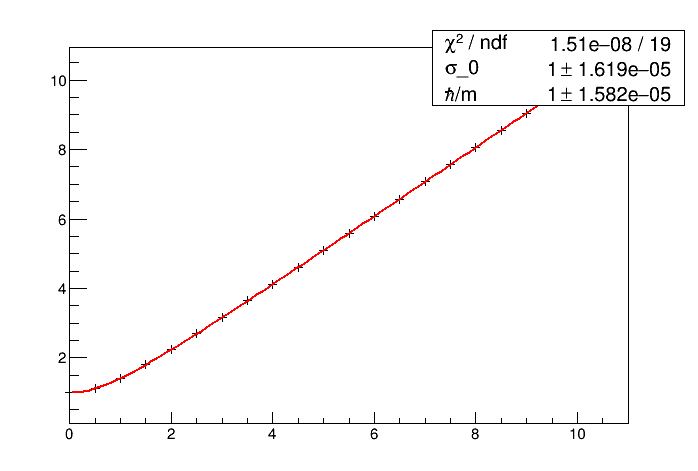
\includegraphics[width=\linewidth]{IMG/dispersione_p}
    \caption{$\sigma_0=1$, $m=1$}
  \end{subfigure}
  ~
  \begin{subfigure}[b]{0.3\textwidth}
    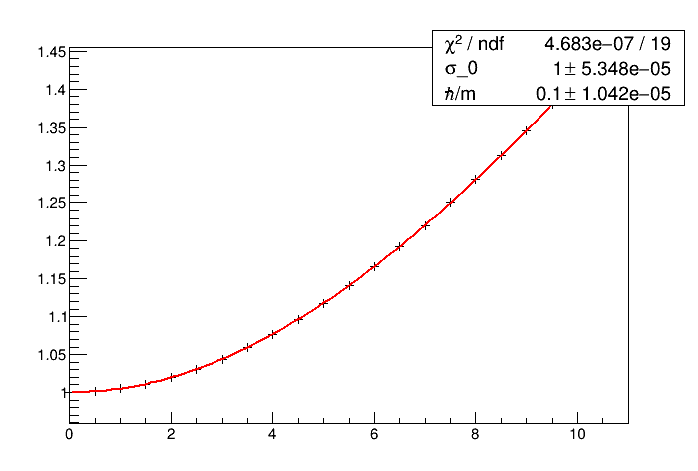
\includegraphics[width=\linewidth]{IMG/dispersione_m10}
    \caption{$\sigma_0=1$, $m=10$}
  \end{subfigure}
  ~
  \begin{subfigure}[b]{0.3\textwidth}
    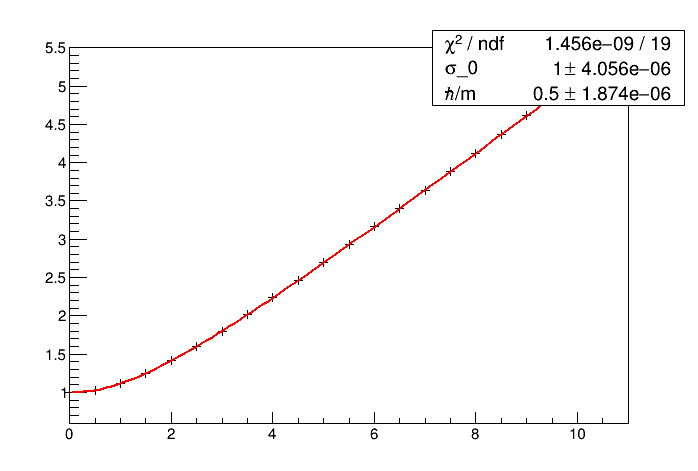
\includegraphics[width=\linewidth]{IMG/dispersione_m2}
    \caption{$\sigma_0=1$, $m=2$}
  \end{subfigure}
  \caption{Alcuni fit dell'andamento della dispersione}\label{fig:dispersioneFitSigma1}
\end{figure}

\begin{figure}[htb]
  \centering
  \begin{subfigure}[b]{0.3\textwidth}
    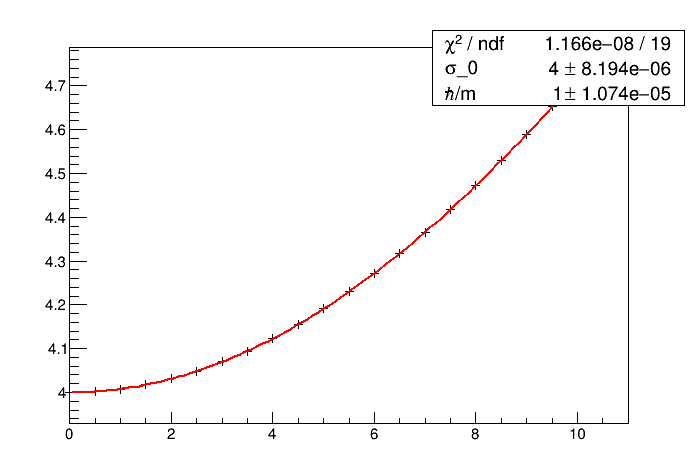
\includegraphics[width=\linewidth]{IMG/dispersione_m1s4}
    \caption{$\sigma_0=4$, $m=1$}
  \end{subfigure}
  ~
  \begin{subfigure}[b]{0.3\textwidth}
    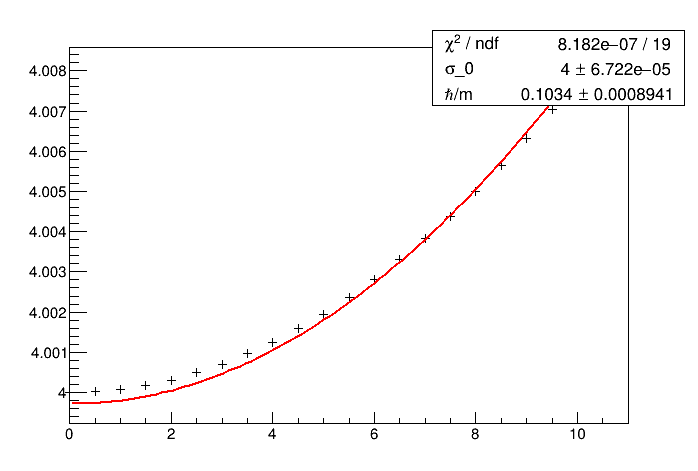
\includegraphics[width=\linewidth]{IMG/dispersione_m10s4}
    \caption{$\sigma_0=4$, $m=10$}
  \end{subfigure}
  ~
  \begin{subfigure}[b]{0.3\textwidth}
    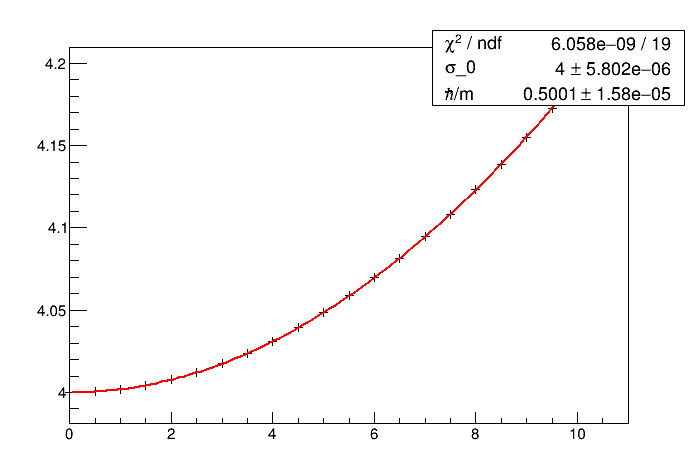
\includegraphics[width=\linewidth]{IMG/dispersione_m2s4}
    \caption{$\sigma_0=4$, $m=2$}
  \end{subfigure}
  \caption{Alcuni fit dell'andamento della dispersione}\label{fig:dispersioneFitSigma4}
\end{figure}

\begin{figure}[htb]
  \centering
  \begin{subfigure}[b]{0.3\textwidth}
    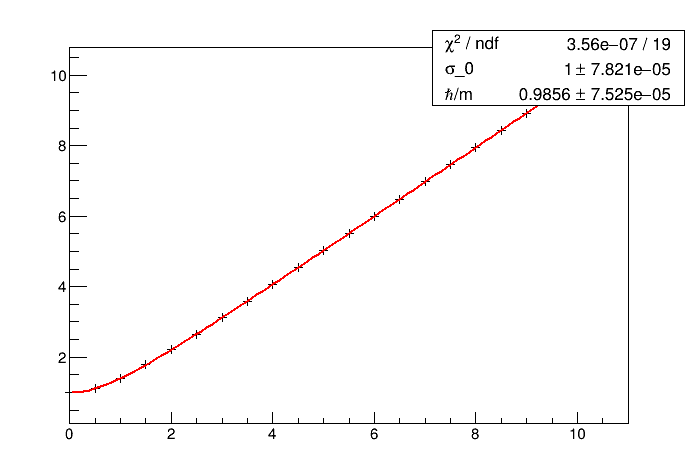
\includegraphics[width=\linewidth]{IMG/dispersione_m1s1e10}
    \caption{$\sigma_0=1$, $m=1$, con $E=10$}
  \end{subfigure}
  ~
  \begin{subfigure}[b]{0.3\textwidth}
    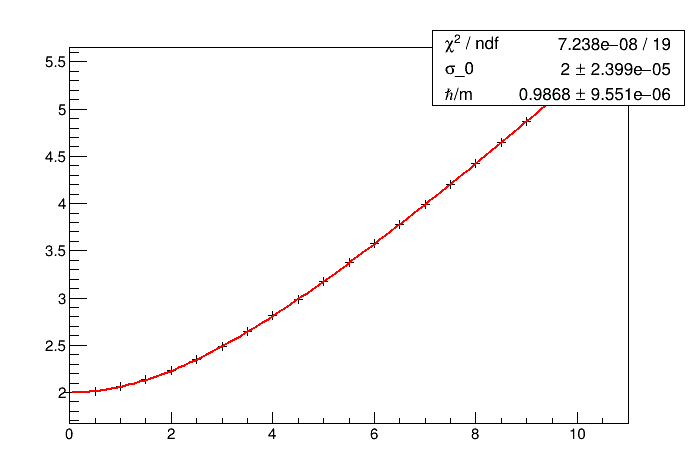
\includegraphics[width=\linewidth]{IMG/dispersione_m1s2e10}
    \caption{$\sigma_0=2$, $m=1$, con $E=10$}
  \end{subfigure}
  ~
  \begin{subfigure}[b]{0.3\textwidth}
    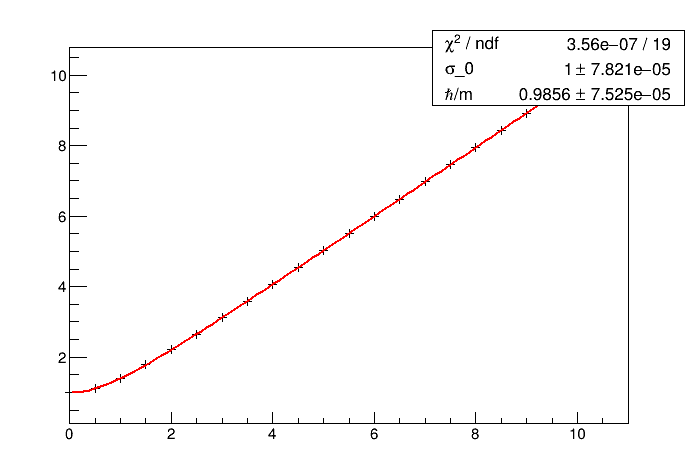
\includegraphics[width=\linewidth]{IMG/dispersione_m1s1e10}
    \caption{$\sigma_0=4$, $m=1$, con $E=10$}
  \end{subfigure}
  \caption{Alcuni fit dell'andamento della dispersione}\label{fig:dispersioneFitE}
\end{figure}

\subsection{La forma delle condizioni iniziali}
Ho effettuato i test precedenti utilizzando come condizione iniziale un pacchetto d'onda gaussiano. Per effetto della dispersione \`e un pacchetto deltiforme che nel tempo si \`e disperso allargandosi in una gaussiana.

Ho provato  ad utilizzare una forma differente per il pacchetto: la funzione ``bump'':
\begin{figure}[hbt]
	\centering
	\begin{tikzpicture}[scale=0.5]
	\begin{axis}[axis x line = center, axis y line = center, xmin = -0.1, xmax = 4.1, ymin=-0.1,ymax =1.5]
	\addplot[domain=-0.1:4.1, samples =501, red]	plot[id=bumpl1]	function{(abs(x-1)<1)? exp(1)*exp(-1/(1-(x-1)*(x-1))):0};
	\addlegendentry{$a=1$, $b=1$}
	\addplot[domain=-0.1:4.1, samples =501, blue]	plot[id=bumpl1]	function{(abs(x-1)<2)? exp(1)*exp(-4/(4-(x-1)*(x-1))):0};
	\addlegendentry{$a=1$, $b=2$}
	\addplot[domain=-0.1:4.1, samples =501, green]	plot[id=bumpl1]	function{(abs(x-3)<1)? exp(-1/(1-(x-3)*(x-3))):0};
	\addlegendentry{$a=3$, $b=1$ non moltiplicata per $e$}
	\end{axis}
	\end{tikzpicture}
	\caption{Alcuni esempi della funzione bump}\label{fig:bump}
\end{figure}

\begin{equation}
bump = \lrt{x} = \lr\{.{\begin{array}{lr}
	e^{-\frac{b^2}{b^2-\lrt{x-a}^2}}&\text{per }\lr||{x-a}<b\\
	0&\text{altrove}
	\end{array}}
\end{equation}

Il ''bump`` \`e una funzione di test quindi \`e definita differente da 0 solo in un intervallo aperto, ed ha la caratteristica di avere tutte le derivate continue, questo mi permetterebbe di ignorare completamente le condizioni al contorno quando la funzione si trova lontano dai bordi della simulazione.
Inoltre moltiplico il risultato per $e$ per avere un pacchetto con il massimo alto $1$, vedi \autoref{fig:bump}.

\begin{figure}[hbt]
	\centering
	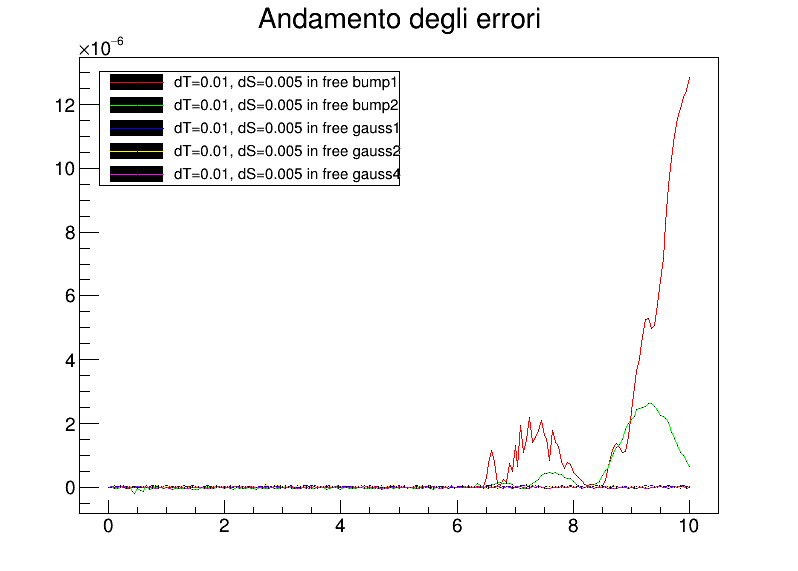
\includegraphics[width=0.5\linewidth]{IMG/testbump}
	\caption[Errore Bump]{l'evoluzione dell'errore del ``bump'' confrontata con quella di un pacchetto gaussiano}\label{fig:testBump}
\end{figure}

A questo punto simulo il pacchetto e confronto l'errore con uno gaussiano. Come si pu\`o vedere dalla \autoref{fig:testBump} non \`e una buona idea.

L'errore cresce molto verso la fine della simulazione, questo potrebbe essere dovuto al fatto che sta impattando contro i limiti del dominio, inoltre se si osserva l'evoluzione della funzione si vede che perde praticamente subito la forma iniziale e quindi anche i vantaggi di avere le code pari a 0.
\begin{figure}[htb]
	\centering
	\begin{subfigure}[b]{0.49\textwidth}
		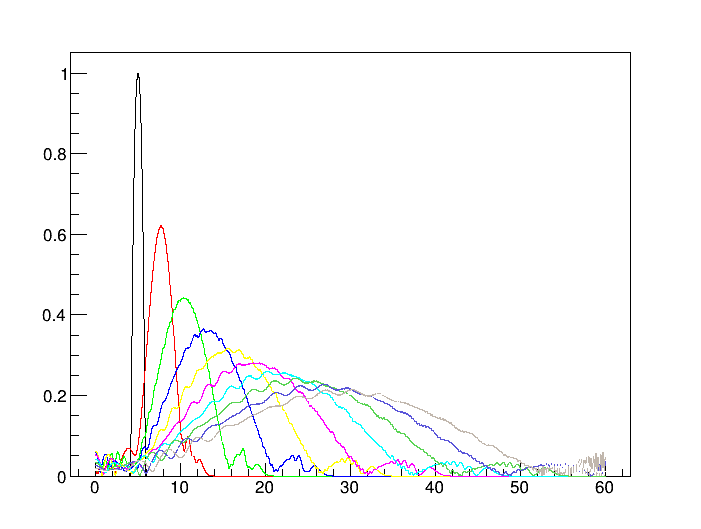
\includegraphics[width=\textwidth]{IMG/bumpDisp1.png}
		\caption{larghezza 1}
	\end{subfigure}
	~
	\begin{subfigure}[b]{0.49\textwidth}
		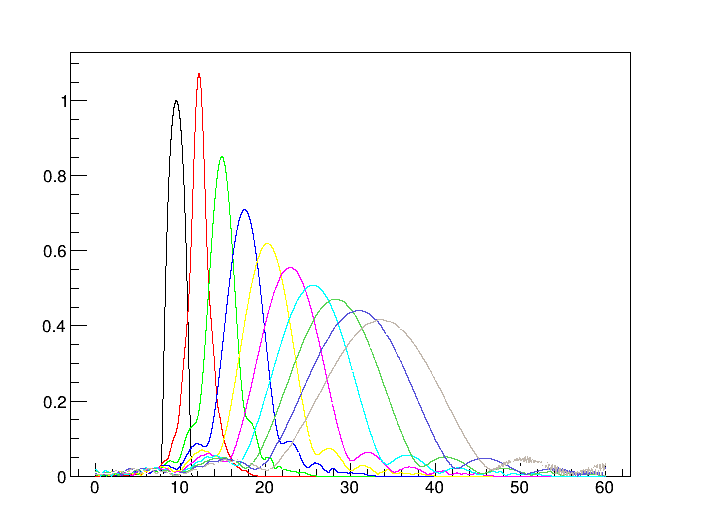
\includegraphics[width=\textwidth]{IMG/bumpDisp2.png}
		\caption{larghezza 2}
	\end{subfigure}
	\caption{L'evoluzione del ``bump'', le ``increspature'' sull'onda che si vedono ai lati sono le figure di interferenza dovute alla riflessione}
\end{figure}

A questo punto l'idea migliore per il pacchetto d'onda sembra essere la gaussiana.


\subsection{Condizioni al contorno}
Quello che vorrei simulare \`e un pacchetto d'onda che sia partito da $-\infty$ e arrivi nel ``punto interessante'', l'area che osservo nella simulazione, e poi prosegua fino all'infinito (o venga eventualmente riflesso).

Per quanto riguarda le condizioni al contorno ho avuto le seguenti idee:
\begin{itemize}
\item Non tengo conto delle condizioni al contorno, faccio in modo di usare pacchetti d'onda ristretti e blocco la simulazione quando questa va ad  avvicinarsi troppo ai bordi.
\item Uso una forma d'onda tale per cui conosco la funzione e la sua derivata in ogni punto
\item Emulo un ambiente chiuso (con ai lati muri di potenziale alti $\infty$)
\end{itemize}
La prima ipotesi \`e stata quella che ho usato in tutte le prove che ho effettuato prima di iniziare a raccogliere dati, considerando 0 il valore della funzione negli estremi.

Per la seconda ipotesi dovrei usare come condizione iniziale una funzione e calcolarne la derivata per ogni passo negli estremi. Ma pacchetti d'onda si disperdono e tendono ad allargarsi, per cui se,  per esempio avessi un pacchetto d'onda generico ($\Psi(x,t) = e^{ikx} \psi(x,t)$), la relazione dovrebbe essere $\partial_x \Psi(x,t) = ik \Psi(x,t) + e^{ikx}\partial_x\psi(x,t)$ e potrei quindi utilizzare le CC di Robin. Ma doveri conoscere come la funzione si disperde nel tempo e ricalcolare quindi  ad ogni passo le condizioni al contorno ed applicarle. Questo per\`o mi porterebbe a svariati problemi quali l'incertezza che la simulazione e la teoria siano esattamente parallele sulla dispersione, il che porterebbe ad altri errori, ed il fatto che molto probabilmente sarebbe poco efficiente dal punto di vista della performance del calcolo.

La terza idea equivale a utilizzare Dirichlet con il valore della funzione pari a 0 nei bordi questo simula un pozzo con pareti di potenziale infinito.

%Per cui ho deciso di ricercare un'idea che simulasse l'assenza di vincoli: ho trovato le cosiddette condizioni al contorno trasparenti.
%Ma ho lasciato perdere data la loro complessit\`a e il poco tempo a mia disposizione, in quanto utilizza la trasformazione Z

\subsection{Prime Conclusioni}
Dopo i primi esperimenti sono arrivato a queste conclusioni:
\begin{itemize}
\item Far\`o le simulazioni utilizzando una gaussiana come forma del pacchetto d'onda, perch\'e mantiene la propria forma.
\item Per contenere la dispersione dell'onda, vista la forma di \eqref{eq:sigmat} posso scegliere di utilizzare un $\sigma_0$ grande oppure una massa grande
  \begin{itemize}
  \item con una massa grande per avere la stessa velocit\`a di gruppo devo aumentare l'energia, ma in compenso posso utilizzare dei $\sigma_0$ piuttosto piccoli e quindi questo mi rende pi\`u semplice il compito di fare confronti tra due parti di spazio limitate per analizzare la trasmissivit\`a delle barriere di potenziale
  \item con $\sigma_0$ grande il pacchetto d'onda  non ha bisogno di una grande energia per muoversi, ma il fatto che esso sia esteso pu\`o comportare problemi per esempio quando si riflette contro un potenziale o quando lo attraversa o nel momento di definire le condizioni iniziali, perch\'e rischio di sovrapporre l'onda al potenziale.
  \end{itemize}
\item Come condizioni al contorno simuler\`o la scatola chiusa con pareti infinite, sebbene una prima idea fosse quella di utilizzare le condizioni ``trasparenti'', ma questo oltre ad appesantire il programma farebbe uscire il pacchetto d'onda dalla mia ``zona d'osservazione'' e quindi non sarei pi\`u in grado di fare l'integrale di tutto il pacchetto (comprese le sue riflessioni e i pezzi in cui si \`e diviso).
\item Per ritardare il pi\`u possibile l'interazione con le condizioni al contorno devo aumentare l'intervallo spaziale se aumento il tempo della simulazione
\item %dire ch eme ne frego del fatto che la velocita` non collima con la teoria
\end{itemize}

Con queste conclusioni in mano mi appresto a simulare le situazioni per cui ho progettato questo algoritmo e confrontarle con la teoria.
